\chapter{Specifikacija programske potpore}
\graphicspath{{./slike/}}		
	\section{Funkcionalni zahtjevi}
			
			\noindent \textbf{Dionici:}
			
			\begin{packed_enum}
				
				\item Vlasnik (naručitelj)
				\item Korisnici
				      \begin{packed_enum}
						
						\item  opći uporabni korisnik 
						\item  administrator aplikacije
						\item administrator satelita
				
					\end{packed_enum}
				\item Razvojni tim
				
			\end{packed_enum}
			
			\noindent \textbf{Aktori i njihovi funkcionalni zahtjevi:}
			
			
			\begin{packed_enum}
				\item  \underbar{Neregistrirani/neprijavljeni korisnik (inicijator) može:}
				
				\begin{packed_enum}
					
					\item se prijaviti u sustav, za što su mu potrebni lozinka (\textit{password}) i korisničko ime (\textit{username})
					
				\end{packed_enum}
			
				\item  \underbar{Obični uporabni korisnik (inicijator) može:}
				
				\begin{packed_enum}
					
					\item se prijaviti u sustav unosom lozinke (\textit{password}) i korisničkog imena (\textit{username}) te promijeniti inicijalo mu dodijeljenu lozinku i korisničko ime
					\item odabrati satelit na kojeg želi poslati poruku i link za komunikaciju 
					\item odlučiti hoće li samostalno odabrati zemeljsku stanicu putem koje se komunicira sa satelitom ili će to sustav napraviti umjesto njega
					\item poslati željeni tekst kao poruku na prethodno odabranu tojku (satelit, link, stanica)
					\item pregledavati i brisati sve poslane poruke i primljene odgovore
					
				\end{packed_enum}
				
				\item  \underbar{Administrator aplikacije (inicijator) može:}
				
				\begin{packed_enum}
					
				    \item kreirati nove korisnike sustava pri čemu im dodijeljue adresu e-pošte (\textit{e-mail}), korisničko ime (\textit{username}), lozinku (\textit{password}) i ulogu (\textit{role})
					\item ostvariti sve funkcionalne zahtjeve običnih uporabnih korisnika
					
				\end{packed_enum}
					\item  \underbar{Administrator satelita (inicijator) može:}
				
				    \begin{packed_enum}
					
				        \item kreirati i izbrisati satelite te promijenjiti njihove parametre
				        \item kreirati i izbrisati linkove te promijenjiti njihove parametre
				        \item kreirati i izbrisati transmitere te promijenjiti njihove parametre
				        \item ostvariti sve funkcionalne zahtjeve običnih uporabnih korisnika
					
				    \end{packed_enum}
				
					\item  \underbar{Baza podataka (sudionik) može:}
				
				\begin{packed_enum}
					
					\item pohraniti sve podatke o korisnicima, njihovim ovlastima i razmijenjenim porukama
					\item pohraniti sve podatke o satelitima, zemaljskim stanicama, linkovima, antenama i transmiterima
					
				\end{packed_enum}
				\item  \underbar{ SatNOGS Network API (sudionik) može:}
				
				\begin{packed_enum}
					
					\item dohvatiti podatke o stanicama i antenama
					
					
				\end{packed_enum}
				\item  \underbar{Satelitte server (sudionik) može:}
			
			\begin{packed_enum}
				
				\item primati poruke koje generira korisnik
				\item odlučiti o prihvaćanju iste poruke
				\item generirati povratnu poruku korisniku
				
				
			\end{packed_enum}
			\end{packed_enum}
			
			\eject 
			
			
				
			\subsection{Obrasci uporabe}

					\noindent \underbar{\textbf{UC1 - Prijava}}
				\begin{packed_item}
					
					\item \textbf{Glavni sudionik: }Neregistrirani korisnik (\textit{guest\_user})
					\item  \textbf{Cilj: }Dobiti pristup korisničkom sučelju
					\item  \textbf{Sudionici: }Baza podataka
				\item \textbf{Preduvjet: }
				\begin{packed_enum}\item Postojanje korisničkog računa u bazi\end{packed_enum}
					\item  \textbf{Opis osnovnog tijeka: }
					
					\item[] \begin{packed_enum}
						
						\item Unos korisničkog imena (\textit{username}) i lozinke (\textit{password})
						\item Sustav potvrđuje ispravnost unesenih podataka
						\item Sustav omogućava pristup korisničkim funkcijama koje definira uloga (\textit{role}) prijavljenog korisnika
						
					\end{packed_enum}
					
					\item  \textbf{Opis mogućih odstupanja: }
					
					\item[] \begin{packed_item}
						
						\item[1] Neispravno korisnicko ime i/ili lozinka
						\item[ ] \begin{packed_enum}
							
							\item[1.1] Sustav obavještava korisnika o neuspjelom upisu i prikazuje\newline prikladnu poruku:  \text "Username or password incorrect"
							
						\end{packed_enum}
						
					\end{packed_item}
				\end{packed_item}
				
				\noindent \underbar{\textbf{UC2 - Pregled osobnih podataka}}
				\begin{packed_item}
					
					\item \textbf{Glavni sudionik: }Korisnik (\textit{user})
					\item  \textbf{Cilj: }Pregledati osobne podatke
					\item  \textbf{Sudionici: }Baza podataka
				\item  \textbf{Preduvjet: }
				\begin{packed_enum}\item Korisnik je prijavljen\end{packed_enum}
					\item  \textbf{Opis osnovnog tijeka: }
					
					\item[] \begin{packed_enum}
					
						\item Korisnik odabire opciju "User details"
						\item Sustav pokazuje osobne podatke korisnika (\textit{username, e-mail} i \textit{ role})
						
					\end{packed_enum}
				\end{packed_item}
				
				\noindent \underbar{\textbf{UC3 - Promjena osobnih podataka}}
				\begin{packed_item}
					
					\item \textbf{Glavni sudionik: }Korisnik (\textit{user})
					\item  \textbf{Cilj: }Promijeniti osobne podatke
					\item  \textbf{Sudionici: }Baza podataka
				\item  \textbf{Preduvjet: }
				\begin{packed_enum}\item Korisnik je prijavljen\end{packed_enum}
					\item  \textbf{Opis osnovnog tijeka: }
					
					\item[] \begin{packed_enum}
						
						\item Korisnik odabere opciju "Edit user details"
						\item Sustav korisniku nudi formu za popunjavanje u kojoj su njegovi trenutni podaci
						\item Korisnik mijenja svoje osobne podatke (\textit{username} i/ili \textit{password})
						\item Korisnik odabere opciju "Save"
						\item Sustav ažurira bazu podataka
						
					\end{packed_enum}
					
					\item  \textbf{Opis mogućih odstupanja: }
					
					\item[] \begin{packed_item}
						
						\item[1] Korisnik promijeni svoje osobne podatke, ali ne odabere opciju "Save"
						\item[ ] \begin{packed_enum}
							
							\item[1.1] Sustav obavještava korisnika da nije spremio podatke prije izlaska iz prozora
							
						\end{packed_enum}
						
						\item[2] Korisnik mijenja \textit{username}, a on je već zauzet
						\item[ ] \begin{packed_enum}
							
							\item[2.1] Sustav obavještava korisnika da je username već zauzet i
							\newline prikazuje prikladnu poruku: "Username already taken"
							
						\end{packed_enum}
						
					\end{packed_item}
				\end{packed_item}
				\noindent \underbar{\textbf{ {\setword{UC4}{Word:UC4}} - Slanje poruke na satelit}}
				\begin{packed_item}
					
					\item \textbf{Glavni sudionik: }Korisnik (\textit{user})
					\item  \textbf{Cilj: }Slanje poruke na odabrani satelit i određivanje parametara
					\item  \textbf{Sudionici: }Baza podataka
					\item  \textbf{Preduvjet: }
					\begin{packed_enum}
					\item Korisnik je prijavljen \item U bazi podataka postoji kompatibilni trio (satelit, link i stanica)	\end{packed_enum}
					\item  \textbf{Opis osnovnog tijeka: }
					
					\item[] \begin{packed_enum}
						
						\item Korisnik odabere opciju za slanje poruke na satelit
						\item Sustav ispisuje listu satelita s nekim njihovim informacijama
						\item Korisnik odabere jedan od satelita
						\item Sustav ispisuje sve podatke o satelitu i njegovim\newline transmiterima
						\item Sustav ispod informacija o satelitu ispisuje listu  kompatibilnih linkova sa svim njihovim informacijama( \textit{frequency}, \textit{mode}, \textit{baud})
						\item Korisnik odabire jedan od linkova
						\item Sustav nudi korisniku opciju da sam odabere željenu stanicu ili da \newline odabir prepusti sustavu
						\item Odabire se kompatibilni satelit ( Vidi \ref{Word:UC5})
						\item {\setword{Sustav vodi korisnika na stranicu s poljem za unošenje teksta poruke}{Word:generiranjem poruke kao što je opisano u UC4}} 
						\item Korisnik unosi poruku i odabire "Send"
						\item Sustav provjerava sa SatNOGS mrežom podudaraju li se naši podaci o \newline odabranoj stanici s trenutnim podacima u njihovoj bazi podataka
						\item Sustav generira sadržaj poruke na temelju vremena slanja, odabranog linka i unesenog teksta
						\item Poruka se označava kao \textit{UPLOAD} i pridružuju joj se parametri komunikacije
						\item Sustav šalje poruku na server(satelit), koji generira povratnu informaciju sličnog formata s oznakom\newline \textit{DOWNLOAD}
						\item Obje poruke se spremaju u bazu podataka s ID oznakom korisnika
						
						
					\end{packed_enum}
					
					\item  \textbf{Opis mogućih odstupanja: }
					
					\item[] \begin{packed_item}
						\item[1] U bazi podataka ne postoji niti jedan satelit
						\item[ ] \begin{packed_enum}
							
							\item[1.1] Sustav obavještava korisnika o nepostojanju satelita
						\end{packed_enum}
					
						\item[2] Poruka poslana na satelit nema definirane sve parametre ili je praznog sadržaja
						\item[ ] \begin{packed_enum}
							
							\item[2.1] Sustav u bazu podataka sprema poruku označenu kao \textit{FAILED UPLOAD}
						\item[2.2] Satelit ne generira povratnu poruku zbog manjka potrebnih informacija o komunikaciji
						\end{packed_enum}	
						\item[3] U bazi podataka ne postoji niti jedan link s odgovarajućim atributima za odabrani satelit
					\item[ ] \begin{packed_enum}
						
						\item[3.1] Sustav obavještava korisnika o nepostojanju odgovarajućeg linka
						\item[3.2] Sustav vraća korisnika na odabir satelita
					\end{packed_enum}		
				\item[4] Sustav je tijekom provjere aktualnosti informacija o stanici, pronašao razliku u podacima bitnim za komunikaciju
				\item[ ] \begin{packed_enum}
					
					\item[4.1] Sustav obavještava korisnika o nemogućnosti slanja poruke odabranim parametrima te ga potiče da pokuša ponovo
					\item[4.2] Sustav osvježava podatke o stanicama i njihovim antenama u bazi podataka
				\end{packed_enum}				
					\end{packed_item}
				\end{packed_item}
			\noindent \underbar{\textbf {\setword{UC5}{Word:UC5} -Biranje stanice}}
			\begin{packed_item}
				
				\item \textbf{Glavni sudionik: }Korisnik (\textit{user})
				\item  \textbf{Cilj: }Odabir zemaljske stanice putem koje se planira poslati poruka
				\item  \textbf{Sudionici: }Baza podataka
				\item  \textbf{Preduvjet: }
				\begin{packed_enum}
					\item Korisnik je prijavljen \item Korisnik je odabrao željeni satelit i link\end{packed_enum}
				\item  \textbf{Opis osnovnog tijeka: }
				
				\item[] \begin{packed_enum}
					
					\item Korisnik ima opciju odabrati "Manual selection" ili "Automatic selection" za odabir stanice
					\item Kod automatskog pretraživanja, sustav odabire stanicu s najvećim brojem obzervacija, koja je kompatibilna s odabranim linkom
					\item Kod ručnog odabira:\begin{itemize}
						\item[a)] Sustav ispisuje listu stanica čije antene podržavaju komunikaciju na način propisan odabranim linkom
						\item[b)] Korisnik odabire stanicu kojom želi poslati poruku
					\end{itemize} 
					\item Nastavljajući proces u \hyperref[Word:generiranjem poruke kao što je opisano u UC4]{UC4} , sustav vodi korisnika na stranicu s poljem za unošenje teksta poruke.
					
				\end{packed_enum}
				
				\item  \textbf{Opis mogućih odstupanja: }
				
				\item[] \begin{packed_item}
				
					\item[1] U bazi podataka ne postoji niti jedna stanica, koja podržava komunikaciju definiranu odabranim linkom
					\item[ ] \begin{packed_enum}
						
						\item[1.1] Sustav obavještava korisnika o nepostojanju adekvatne stanice
						\item[1.2] Sustav vraća korisnika na ponovni izbor satelita( Vidi \ref{Word:UC4})
					\end{packed_enum}
								
					
				\end{packed_item}
			\end{packed_item}
				\noindent \underbar{\textbf{UC6 - Pregled poslanih zahtjeva i rezultata}}
				\begin{packed_item}
					
					\item \textbf{Glavni sudionik: }Korisnik (\textit{user})
					\item  \textbf{Cilj: }Pregled vlastitih komunikacija putem mreže
					\item  \textbf{Sudionici: }Baza podataka
					\item  \textbf{Preduvjet: }
					\begin{packed_enum}\item Korisnik je prijavljen\end{packed_enum}
					\item  \textbf{Opis osnovnog tijeka: }
					
					\item[] \begin{packed_enum}
						
						\item Korisnik odabere opciju "Message history"
						\item Sustav ispisuje tablicu prošlih komunikacija korisnika
						\item U tablici korisnik može vidjeti tekst poruke, vrijeme slanja poruke, smjer komunikacije (\textit{UPLOAD}/\textit{DOWNLOAD}/\textit{FAILED UPLOAD}), imena satelita i stanice putem koje se komuniciralo te informacije o korištenom linku
						
					\end{packed_enum}
					
					\item  \textbf{Opis mogućih odstupanja: }
					
					\item[] \begin{packed_item}
						
						\item[1] Korisnik nema nikakvih prijašnjih poruka
						\item[ ] \begin{packed_enum}
							
							\item[1.1] Sustav obavještava korisnika o nepostojanju prijašnje komunikacije sa satelitima
							
						\end{packed_enum}
					
					\end{packed_item}
				\end{packed_item}
				
				
					\noindent \underbar{\textbf{UC7 - Brisanje poslanih zahtjeva}}
				\begin{packed_item}
					
					\item \textbf{Glavni sudionik: }Korisnik (\textit{user})
					\item  \textbf{Cilj: }Brisanje kompletne povjesti vlastitih poruka
					\item  \textbf{Sudionici: }Baza podataka
						\item  \textbf{Preduvjet: }
					\begin{packed_enum}
						\item Korisnik je prijavljen \item Korisnik u bazi ima zabilježenu barem jednu poruku	\end{packed_enum}
					\item  \textbf{Opis osnovnog tijeka: }
					
					\item[] \begin{packed_enum}
						
						\item Korisnik odabere opciju "Erase all"
						\item Sustav provjerava je li korisnik siguran da želi obrisati sve poruke
						\item Sustav iz baze briše sve poruke povezane s korisnikom
						
					\end{packed_enum}
					
					\item  \textbf{Opis mogućih odstupanja: }
					
					\item[] \begin{packed_item}
						
							\item[1] korisnik odabere opciju za brisanje, ali odustane od brisanja kod potvrde
						\item[ ] \begin{packed_enum}
							
							\item[1.1]Sustav obavještava Korisnika da se brisanje nije dogodilo				
						\end{packed_enum}
						
					\end{packed_item}
				\end{packed_item}
			\noindent \underbar{\textbf{UC8 - Pregled korisnika}}
			\begin{packed_item}
				
				\item \textbf{Glavni sudionik: }Administrator stranice (\textit{super\_admin})
				\item  \textbf{Cilj: }Pregledati popis korisnika i njihovih podataka
				\item  \textbf{Sudionici: }Baza podataka
				\item  \textbf{Preduvjet: }
				\begin{packed_enum}\item Korisnik je prijavljen kao administrator stranice\end{packed_enum}
				\item  \textbf{Opis osnovnog tijeka: }
				
				\item[] \begin{packed_enum}
					
					\item Administrator stranice odabere opciju "Users"
					\item Sustav ispisuje listu svih ostalih korisnika s njihovim osobnim\newline podacima
					
				\end{packed_enum}
				
				\item  \textbf{Opis mogućih odstupanja: }
				
				\item[] \begin{packed_item}
					
					\item[1] Ne postoje drugi korisnici
					\item[ ] \begin{packed_enum}
						
						\item[1.1] Sustav Ispod prazne tablice korisnika ispisuje obavijest:\newline "Application has no other users."
						
					\end{packed_enum}
					
				\end{packed_item}
			\end{packed_item}
			
				\noindent \underbar{\textbf{UC9 - Brisanje odabranog korisnika}}
				\begin{packed_item}
					
					\item \textbf{Glavni sudionik: }Administrator stranice (\textit{super\_admin})
					\item  \textbf{Cilj: }Izbrisati podatke o korisniku iz baze podataka
					\item  \textbf{Sudionici: }Baza podataka
					\item  \textbf{Preduvjet: }
					\begin{packed_enum}
						 \item Korisnik je prijavljen kao administrator stranice\item  Postoji barem jedan drugi korisnik u bazi podataka	\end{packed_enum}
					\item  \textbf{Opis osnovnog tijeka: }
					
					\item[] \begin{packed_enum}
						
						\item Administrator stranice odabere željenog korisnika na listi korisnika
						\item Administrator stranice odabere opcije "Erase"
						\item Administrator stranice potvrđuje svoj odabir
						\item Sustav briše podatke u bazi vezane uz korisnika\newline (osobni podaci i zabilježene poruke)
						
					\end{packed_enum}
					
					\item  \textbf{Opis mogućih odstupanja: }
					
					\item[] \begin{packed_enum}
						
						\item[1] Administrator stranice odabere korisnika, ali odustane od brisanja kod potvrde
						\item[ ] \begin{packed_enum}
							
							\item[1.1]Sustav obavještava administratora da se brisanje nije dogodilo
					\end{packed_enum}
				\end{packed_enum}
					\end{packed_item}
					\noindent \underbar{\textbf{UC10 - Dodavanje novog korisnika}}
				\begin{packed_item}
					
					\item \textbf{Glavni sudionik: }Administrator stranice (\textit{super\_admin})
					\item  \textbf{Cilj: }Kreiranje i dodavanje novog korisnika
					\item  \textbf{Sudionici: }Baza podataka
					\item  \textbf{Preduvjet: }
					\begin{packed_enum}
						\item Korisnik je prijavljen kao administrator stranice	\end{packed_enum}
					\item  \textbf{Opis osnovnog tijeka: }
					
					\item[] \begin{packed_enum}
						
						\item Administrator stranice odabere opciju "Add new user" 
						\item Susatav administratoru nudi formu za popunjavanje
						\item Administrator stranice unosi osnovne podatke o novom\newline korisniku (\textit{ username}, \textit{e-mail}, \textit{password} i \textit{role})
						\item Administrator stranice odabere opciju "Create"
						\item Sustav u bazi podataka stvara novog korisnika
						
					\end{packed_enum}
					
					\item  \textbf{Opis mogućih odstupanja: }
					
					\item[] \begin{packed_enum}
						
						\item[1] Administrator stranice odabere \textit{e-mail}  koji već koristi neki drugi korisnik
						\item[ ] \begin{packed_enum}
							
							\item[1.1] Sustav provjerava jednistvenost ovih podataka u bazi i vraća\newline Administratora stranice na unos podataka s porukom o pogrešci:\newline "E-mail already in use"
						\end{packed_enum}
					\item[2] Administrator stranice odabere \textit{username} koji već koristi neki drugi korisnik
					\item[ ] \begin{packed_enum}
						
						\item[2.1] Sustav provjerava jednistvenost ovih podataka u bazi i vraća\newline Administratora stranice na unos podataka s porukom o pogrešci:\newline "Username already in use"
					\end{packed_enum}
					\end{packed_enum}
				\end{packed_item}
			
			\noindent \underbar{\textbf{\setword{UC11}{UC11} - Prikaz liste transmitera}}
			\begin{packed_item}
				
				\item \textbf{Glavni sudionik: }Administrator satelita (\textit{satellite\_admin})
				\item  \textbf{Cilj: }Pregled liste već postojećih transmitera
				\item  \textbf{Sudionici: }Baza podataka
				\item  \textbf{Preduvjet: }
				\begin{packed_enum}
					\item Korisnik je prijavljen kao administrator satelita	\end{packed_enum}
				\item  \textbf{Opis osnovnog tijeka: }
				
				\item[] \begin{packed_enum}
					
					\item Administrator satelita odabere opciju "Transmitters"
					\item Sustav ispisuje listu transmitera i njihovih atributa (\textit{name}, \textit{frequency}, \textit{mode} i \textit{baud})
					\item Aministrator satelita može odabrati pojedini transmiter( Vidi \hyperref[UC24] {UC24})
					
				\end{packed_enum}
				
				\item  \textbf{Opis mogućih odstupanja: }
				
				\item[] \begin{packed_enum}
					
					\item[1] U bazi podataka ne postoji niti jedan transmiter
					\item[ ] \begin{packed_enum}
						
						\item[1.1] Sustav Ispod prazne tablice transmitera ispisuje obavijest:\newline "Application has no registered Transmiters." 
					\end{packed_enum}
				\end{packed_enum}
			\end{packed_item}
			\noindent \underbar{\textbf{\setword{UC12}{UC12} - Dodavanje novog transmitera}}
			\begin{packed_item}
				
				\item \textbf{Glavni sudionik: }Administrator satelita (\textit{satellite\_admin})
				\item  \textbf{Cilj: }Stvaranje novog transmitera
				\item  \textbf{Sudionici: }Baza podataka
				\item  \textbf{Preduvjet: }
				\begin{packed_enum}
					\item Korisnik je prijavljen kao administrator satelita	\end{packed_enum}
				\item  \textbf{Opis osnovnog tijeka: }
				
				\item[] \begin{packed_enum}
					\item Administratr satelita odabere opciju "Add Transmiter"
					\item Sustav administratoru nudi formu za popunjavanje podataka
					\item Administrator satelita unosi podatke o novom transmiteru(\textit{name}, \textit{frequency}, \textit{mode} i \textit{baud})
					\item Administrator satelita odabere opciju "Submit"
					\item Sustav kreira novi zapis u bazi podataka na temelju unesenih podataka.
					\item Ako postoji link s identičnim atributima, sustav zapisuje \textit{linkId}  tog linka u naš zapis
					\item Sustav vraća administratora na prikaz satelita (Vidi \hyperref[UC26]{  UC26})
					
				\end{packed_enum}
				
				\item  \textbf{Opis mogućih odstupanja: }
				
				\item[] \begin{packed_enum}
					
					\item[1] U bazi podataka postoji transmiter koji ima isto ime
					\item[ ] \begin{packed_enum}
						
						\item[1.1] Sustav ne dozvoljava korisniku da pritisne "Submit"
						\item[1.2] Sustav obavještava administratora porukom "Transmitter with this name already exists"
					\end{packed_enum}
				\end{packed_enum}
			\end{packed_item}
			\noindent \underbar{\textbf{\setword{UC13}{UC13} - Brisanje transmitera}}
			\begin{packed_item}
				
				\item \textbf{Glavni sudionik: }Administrator satelita (\textit{satellite\_admin})
				\item  \textbf{Cilj: }Brisanje postojećeg transmitera
				\item  \textbf{Sudionici: }Baza podataka
				\item  \textbf{Preduvjet: }
				\begin{packed_enum}
					\item Korisnik je prijavljen kao administrator satelita
					\item Postoji barem jedan transmiter u bazi podataka	\end{packed_enum}
				\item  \textbf{Opis osnovnog tijeka: }
				
				\item[] \begin{packed_enum}
					
					\item Administrator satelita odabere opciju "Delete" na odabranom transmiteru
					\item Sustav provjerava je li administator siguran da želi obrisati transmiter
					\item Sustav iz baze briše sve podatke o transmiteru 
					\item Sustav vraća Administratora na \hyperref[UC11]{prikaz liste transmitera (Vidi UC11) } 
					
				\end{packed_enum}
				
				\item  \textbf{Opis mogućih odstupanja: }
				
				\item[] \begin{packed_enum}
					
					\item[1] Administrator stranice odabere transmiter, ali odustane od brisanja kod potvrde
					\item[ ] \begin{packed_enum}
						
						\item[1.1] Sustav obavještava administratora da se brisanje nije dogodilo
					\end{packed_enum}
				\end{packed_enum}
			\end{packed_item}
			\noindent \underbar{\textbf{\setword{UC14}{UC14} - Promjena parametara transmitera}}
			\begin{packed_item}
				
				\item \textbf{Glavni sudionik: }Administrator satelita (\textit{satellite\_admin})
				\item  \textbf{Cilj: }Promjena parametara transmitera
				\item  \textbf{Sudionici: }Baza podataka
				\item  \textbf{Preduvjet: }
				\begin{packed_enum}
					\item Korisnik je prijavljen kao administrator satelita
					\item U bazi postoji barem jedan transmiter \end{packed_enum}
				\item  \textbf{Opis osnovnog tijeka: }
				
				\item[] \begin{packed_enum}
					\item Administratr satelita odabere opciju "Edit"
					\item Sustav administratoru nudi formu za popunjavanje u kojoj su trenutni podaci o transmiteru
					\item Administrator satelita mijenja podatke o transmiteru (\textit{name}, \textit{frequency}, \textit{mode} i \textit{baud})
					\item Administrator satelita odabere opciju "Submit"
					\item Sustav mijenja zapis u bazi podataka na temelju unesenih podataka
					
				\end{packed_enum}
				
				\item  \textbf{Opis mogućih odstupanja: }
				
				\item[] \begin{packed_enum}
					
					\item[1] U bazi podataka postoji drugi transmiter koji ima isto ime
					\item[ ] \begin{packed_enum}
						
						\item[1.1] Sustav ne dozvoljava korisniku da pritisne "Submit"
						\item[1.2] Sustav obavještava administratora porukom "Transmitter with this name already exists"
					\end{packed_enum}
				\end{packed_enum}
			\end{packed_item}
			
			\noindent \underbar{\textbf{\setword{UC15}{UC15} - Prikaz liste linkova}}
			\begin{packed_item}
				
				\item \textbf{Glavni sudionik: }Administrator satelita (\textit{satellite\_admin})
				\item  \textbf{Cilj: }Pregled liste već postojećih linkova
				\item  \textbf{Sudionici: }Baza podataka
				\item  \textbf{Preduvjet: }
				\begin{packed_enum}
					\item Korisnik je prijavljen kao administrator satelita	\end{packed_enum}
				\item  \textbf{Opis osnovnog tijeka: }
				
				\item[] \begin{packed_enum}
					
					\item Administrator satelita odabere opciju "Links"
					\item Sustav ispisuje listu linkova i njihovih atributa(\textit{frequency}, \textit{ mode} i \textit{baud})
					\item Aministrator satelita može odabrati pojedini link( Vidi \hyperref[UC25] {UC25})
					
					\item Iznad same tablice Administratoru satelita se nudi opcija \hyperref[UC16]{"Add Link"}
					
				\end{packed_enum}
				
				\item  \textbf{Opis mogućih odstupanja: }
				
				\item[] \begin{packed_enum}
					
					\item[1] U bazi podataka ne postoji niti jedan link
					\item[ ] \begin{packed_enum}
						
						\item[1.1] Sustav ispod prazne tablice linkova ispisuje obavijest:\newline "Application has no registered Links." 
					\end{packed_enum}
				\end{packed_enum}
			\end{packed_item}
			\noindent \underbar{\textbf{\setword{UC16}{UC16} - Dodavanje novog linka}}
		\begin{packed_item}
			
			\item \textbf{Glavni sudionik: }Administrator satelita (\textit{satellite\_admin})
			\item  \textbf{Cilj: }Stvaranje novog linka
			\item  \textbf{Sudionici: }Baza podataka
			\item  \textbf{Preduvjet: }
			\begin{packed_enum}
				\item Korisnik je prijavljen kao administrator satelita	\end{packed_enum}
			\item  \textbf{Opis osnovnog tijeka: }
			
			\item[] \begin{packed_enum}
				\item Administrator satelita odabere opciju "Add Link"
				\item Sustav administratoru nudi formu za popunjavanje podataka
				\item Administrator satelita unosi podatke o novom linku( \textit{frequency}, \textit{mode}, \textit{baud})
				\item Administrator satelita odabere opciju "Submit"
				\item Sustav kreira novi zapis u bazi podataka na temelju unesenih podataka i administratorovog Id-a
				\item Sustav vraća administratora na \hyperref[UC15]{prikaz liste linkova (Vidi UC15)} 
				
			\end{packed_enum}
			
			\item  \textbf{Opis mogućih odstupanja: }
			
			\item[] \begin{packed_enum}
				
				\item[1] U bazi podataka postoji link koji sadrži iste podatke za sva tri unesena podatka
				\item[ ] \begin{packed_enum}
					
					\item[1.1] Sustav ne dozvoljava korisniku da pritisne "Submit"
					\item[1.2] Sustav obavještava administratora porukom "Link with these atributes already exists"
				\end{packed_enum}
			\end{packed_enum}
		\end{packed_item}
					\noindent \underbar{\textbf{\setword{UC17}{UC17} - Brisanje linka}}
				\begin{packed_item}
					
					\item \textbf{Glavni sudionik: }Administrator satelita (\textit{satellite\_admin})
					\item  \textbf{Cilj: }Brisanje postojećeg linka
					\item  \textbf{Sudionici: }Baza podataka
					\item  \textbf{Preduvjet: }
					\begin{packed_enum}
						\item Korisnik je prijavljen kao administrator satelita
						\item Postoji barem jedan link u bazi podataka	\end{packed_enum}
					\item  \textbf{Opis osnovnog tijeka: }
					
					\item[] \begin{packed_enum}
						
						\item Administrator satelita odabere opciju "Delete" na odabranom linku
						\item Sustav provjerava je li administrator siguran da želi obrisati link 
						\item Sustav u bazi podataka briše sve podatke o linku 
						\item Sustav vraća administratora na \hyperref[UC15]{prikaz liste linkova (Vidi UC15)} 
						
					\end{packed_enum}
					
					\item  \textbf{Opis mogućih odstupanja: }
					
					\item[] \begin{packed_enum}
						
							\item[1] Administrator odabere link, ali odustane od brisanja kod potvrde
						\item[ ] \begin{packed_enum}
							
							\item[1.1] Sustav obavještava administratora da se brisanje nije dogodilo
						\end{packed_enum}
					\end{packed_enum}
				\end{packed_item}
				\noindent \underbar{\textbf{\setword{UC18}{UC18} - Promjena parametara linka}}
			\begin{packed_item}
				
				\item \textbf{Glavni sudionik: }Administrator satelita (\textit{satellite\_admin})
				\item  \textbf{Cilj: }Promjena parametara linka
				\item  \textbf{Sudionici: }Baza podataka
				\item  \textbf{Preduvjet: }
				\begin{packed_enum}
					\item Korisnik je prijavljen kao administrator satelita
				\item U bazi postoji barem jedan link	\end{packed_enum}
				\item  \textbf{Opis osnovnog tijeka: }
				
				\item[] \begin{packed_enum}
					\item Administratr satelita odabere opciju "Edit"
					\item Sustav administratoru nudi formu za popunjavanje u kojoj su trenutni podaci o linku
					\item Administrator satelita mijenja podatke o linku( \textit{frequency}, \textit{mode}, \textit{baud})
					\item Administrator satelita odabere opciju  "Submit"
					\item Sustav mijenja zapis u bazi podataka na temelju unešenih podataka
					\item Sustav vraća administratora na \hyperref[UC15]{prikaz liste linkova (Vidi UC15)} 
					
				\end{packed_enum}
				
				\item  \textbf{Opis mogućih odstupanja: }
				
				\item[] \begin{packed_enum}
					
					\item[1] U bazi podataka postoji link s drugim \textit{linkId}-em koji sadrži iste parametre
					\item[ ] \begin{packed_enum}
						
						\item[1.1] Sustav ne dozvoljava korisniku da pritisne "Submit"
						\item[1.2] Sustav obavještava administratora porukom "Link with these atributes already exists"
					\end{packed_enum}
				\end{packed_enum}
			\end{packed_item}

 \noindent \underbar{\textbf{\setword{UC19}{UC19} - Prikaz liste satelita}}
			\begin{packed_item}
				
				\item \textbf{Glavni sudionik: }Administrator satelita (\textit{satellite\_admin})
				\item  \textbf{Cilj: }Pregled liste već postojećih satelita
				\item  \textbf{Sudionici: }Baza podataka
				\item  \textbf{Preduvjet: }
				\begin{packed_enum}
					\item Korisnik je prijavljen kao administrator satelita	\end{packed_enum}
				\item  \textbf{Opis osnovnog tijeka: }
				
				\item[] \begin{packed_enum}
					
					\item Administrator satelita odabere opciju "Satellites"
					\item Sustav ispisuje popis postojećih satelita te njihove osnovne atribute 
					\item Administrator može kliknuti na zapis satelita u prikazanoj tablici i svi njegovi podaci će biti prikazani ( Vidi \hyperref[UC26] {UC26})
					\item Iznad same tablice administratoru satelita se nudi opcija \hyperref[UC20]{ "Add Satellite"}
					
				\end{packed_enum}
				
				\item  \textbf{Opis mogućih odstupanja: }
				
				\item[] \begin{packed_enum}
					
					\item[1] U bazi podataka ne postoji niti jedan satelit
					\item[ ] \begin{packed_enum}
						
						\item[1.1] Sustav ispod prazne tablice linkova ispisuje obavijest:\newline "Application has no registered Satellites." 
					\end{packed_enum}
				\end{packed_enum}
			\end{packed_item}
			\noindent \underbar{\textbf{\setword{UC20}{UC20} - Dodavanje novog satelita}}
		\begin{packed_item}
			
			\item \textbf{Glavni sudionik: }Administrator satelita (\textit{satellite\_admin})
			\item  \textbf{Cilj: }Stvaranje novog satelita
			\item  \textbf{Sudionici: }Baza podataka
			\item  \textbf{Preduvjet: }
			\begin{packed_enum}
				\item Korisnik je prijavljen kao administrator satelita	\end{packed_enum}
			\item  \textbf{Opis osnovnog tijeka: }
			
			\item[] \begin{packed_enum}
				\item Administratr satelita odabere opciju "Add satellite"
				\item Sustav Administratoru nudi formu za popunjavanje podataka
				\item Administrator satelita unosi podatke o novom satelitu (\textit{name})
				\item Administrator satelita odabere opciju "Submit"
				\item Sustav kreira novi zapis u bazi podataka na temelju unesenih podataka i Administratorovog Id-a
				\item Sustav vraća Administratora na \hyperref[UC19]{prikaz liste satelita } 
				
			\end{packed_enum}
			
			\item  \textbf{Opis mogućih odstupanja: }
			
			\item[] \begin{packed_enum}
				
				\item[1] U bazi podataka postoji satelit koji ima isto ime
				\item[ ] \begin{packed_enum}
					
					\item[1.1] Sustav ne dozvoljava korisniku da pritisne "Submit"
					\item[1.2] Sustav obavještava administratora porukom "Satellite with this name already exists"
				\end{packed_enum}
			\end{packed_enum}
		\end{packed_item}
					\noindent \underbar{\textbf{\setword{UC21}{UC21} - Brisanje satelita}}
				\begin{packed_item}
					
					\item \textbf{Glavni sudionik: }Administrator satelita (\textit{satellite\_admin})
					\item  \textbf{Cilj: }Brisanje postojećeg satelita
					\item  \textbf{Sudionici: }Baza podataka
					\item  \textbf{Preduvjet: }
					\begin{packed_enum}
						\item Korisnik je prijavljen kao administrator satelita
						\item Postoji barem jedan satelit u bazi podataka	\end{packed_enum}
					\item  \textbf{Opis osnovnog tijeka: }
					
					\item[] \begin{packed_enum}
						
						\item Administrator satelita odabire opciju "Delete" na odabranom satelitu
						\item Sustav provjerava je li administator siguran da želi obrisati satelit
						\item Sustav iz baze podataka briše sve podatke o satelitu 
						\item Sustav vraća administratora na \hyperref[UC19]{prikaz liste satelita (Vidi UC19) } 
						
					\end{packed_enum}
					
					\item  \textbf{Opis mogućih odstupanja: }
					
					\item[] \begin{packed_enum}
						
							\item[1] Administrator satelita odabere satelit, ali odustane od brisanja kod potvrde
						\item[ ] \begin{packed_enum}
							
							\item[1.1] Sustav obavještava administratora da se brisanje nije dogodilo
						\end{packed_enum}
					\end{packed_enum}
				\end{packed_item}
				\noindent \underbar{\textbf{\setword{UC22}{UC22} - Promjena parametara satelita}}
			\begin{packed_item}
				
				\item \textbf{Glavni sudionik: }Administrator satelita (\textit{satellite\_admin})
				\item  \textbf{Cilj: }Promjena parametara satelita
				\item  \textbf{Sudionici: }Baza podataka
				\item  \textbf{Preduvjet: }
				\begin{packed_enum}
					\item Korisnik je prijavljen kao administrator satelita
				\item U bazi postoji barem jedan satelit	\end{packed_enum}
				\item  \textbf{Opis osnovnog tijeka: }
				
				\item[] \begin{packed_enum}
					\item Administrator satelita odabere opciju "Edit"
					\item Sustav administratoru nudi formu za popunjavanje u kojoj su trenutni podaci o satelitu
					\item Administrator satelita mijenja podatke o satelitu (\textit{name})
					\item Administrator satelita odabere opciju "Submit"
					\item Sustav mijenja zapis u bazi podataka na temelju unesenih podataka
					\item Sustav vraća administratora na \hyperref[UC19]{prikaz liste satelita (Vidi UC19)} 
					
				\end{packed_enum}
				
				\item  \textbf{Opis mogućih odstupanja: }
				
				\item[] \begin{packed_enum}
					
					\item[1] U bazi podataka postoji satelit sa drugim \textit{satelliteId}-em koji sadrži isto ime
					\item[ ] \begin{packed_enum}
						
						\item[1.1] Sustav ne dozvoljava korisniku da pritisne "Submit"
						\item[1.2] Sustav obavještava administratora porukom "Satellite with this name already exists"
					\end{packed_enum}
				\end{packed_enum}
			\end{packed_item}
		
		 
		
		
		
		\noindent \underbar{\textbf{UC23 - Osvježavanje informacija o stanicama}}
		\begin{packed_item}
			
			\item \textbf{Glavni sudionik: }Baza podataka (\textit{Data base})
			\item  \textbf{Cilj: }Osvježavanje tablice stanica i tablice antena
			\item  \textbf{Sudionici: }Satnogs network api
			\item  \textbf{Preduvjet: }
			\begin{packed_enum}
				\item Vrijeme sustava je ponoć(00:00)	\end{packed_enum}
			\item  \textbf{Opis osnovnog tijeka: }
			
			\item[] \begin{packed_enum}
				
				\item Sustav se spaja na SatNOGS Network API
				\item Sustav briše sve podatke o satelitima i antenama iz baze podataka \newline(ukljućujući tablice linkAntenna i statAntenna)
				\item Sustav šalje Get zahtjev za stanice SatNOGS Network API-ju
				\item SatNOGS Network API vraća listu stanica sa svim njihovim atributima
				\item Sustav parsira podatke o svakoj stanici i stvara njihove zapise: ( \textit{Id, name, number of observations, latitude, longitude, altitude} i \textit{status})
				\item Sustav također na temelju podataka o anteni stvara nove zapise o\newline antenama (\textit{type, min frequency, max frequency})
				\item Sustav pohranjuje nove podatke u bazu podataka
				
				
			\end{packed_enum}
			
			\item  \textbf{Opis mogućih odstupanja: }
			
			\item[] \begin{packed_enum}
				
				\item[1] Sustav se ne uspijeva spojiti na  SatNOGS Network API
				\item[ ] \begin{packed_enum}
					
					\item[1.1] Sustav prekida s procesom osvježavanja tablica
					\item[1.2] Sustav pokušava ponoviti proces sljedećeg dana u ponoć(00:00)
				\end{packed_enum}
			\end{packed_enum}
		\end{packed_item}
	\noindent \underbar{\textbf{\setword{UC24}{UC24} - Prikaz transmitera}}
	\begin{packed_item}
		
		\item \textbf{Glavni sudionik: }Administrator satelita (\textit{satellite\_admin})
		\item  \textbf{Cilj: }Pregled postojećeg transmitera
		\item  \textbf{Sudionici: }Baza podataka
		\item  \textbf{Preduvjet: }
		\begin{packed_enum}
			\item Korisnik je prijavljen kao administrator satelita	\end{packed_enum}
		\item  \textbf{Opis osnovnog tijeka: }
		
		\item[] \begin{packed_enum}
					
			\item Sustav ispisuje atribute transmitera (\textit{name}, \textit{frequency}, \textit{mode} i \textit{baud}) i satelit na kojem se transmiter nalazi
			\item U kutu postoje dvije opcije (\hyperref[UC14]{ "Edit"} i \hyperref[UC13]{ "Delete"})
			
			
		\end{packed_enum}
	\end{packed_item}
\noindent \underbar{\textbf{\setword{UC25}{UC25} - Prikaz linka}}
\begin{packed_item}
	
	\item \textbf{Glavni sudionik: }Administrator satelita (\textit{satellite\_admin})
	\item  \textbf{Cilj: }Pregled postojećeg linka
	\item  \textbf{Sudionici: }Baza podataka
	\item  \textbf{Preduvjet: }
	\begin{packed_enum}
		\item Korisnik je prijavljen kao administrator satelita	\end{packed_enum}
	\item  \textbf{Opis osnovnog tijeka: }
	
	\item[] \begin{packed_enum}
		
		\item Sustav ispisuje atribute linka (\textit{frequency}, \textit{mode} i \textit{baud})
		\item U kutu postoje dvije opcije (\hyperref[UC18]{ "Edit"} i \hyperref[UC17]{ "Delete"})
		
		
	\end{packed_enum}
\end{packed_item}

\noindent \underbar{\textbf{\setword{UC26}{UC26} - Prikaz satelita}}
\begin{packed_item}
	
	\item \textbf{Glavni sudionik: }Administrator satelita (\textit{satellite\_admin})
	\item  \textbf{Cilj: }Pregled postojećeg satelita
	\item  \textbf{Sudionici: }Baza podataka
	\item  \textbf{Preduvjet: }
	\begin{packed_enum}
		\item Korisnik je prijavljen kao administrator satelita
			\end{packed_enum}
	\item  \textbf{Opis osnovnog tijeka: }
	
	\item[] \begin{packed_enum}
		
		\item Sustav ispisuje osnovne atribute satelita
		\item U kutu postoje dvije opcije (\hyperref[UC22]{ "Edit"} i \hyperref[UC21]{ "Delete"})
		\item Ispod tih informacija sustav ispisuje listu transmitera povezanih s ovim satelitom i njihove informacije
		\item Iznad transmitera nalazi se opcija za dodavanje transmitera(\hyperref[UC12]{ "Add transmitter"})
		\item Administrator ima opciju odabrati jedan transmiter i pristupiti njegovim podacima( Vidi\hyperref[UC24]{ UC24})
		
	\end{packed_enum}
\end{packed_item}
	
				
				
				\newpage
				\subsubsection{Dijagrami obrazaca uporabe}
					\begin{figure}[H]
						\label{fig:Dijagrami obrazaca uporabe 1-7}
						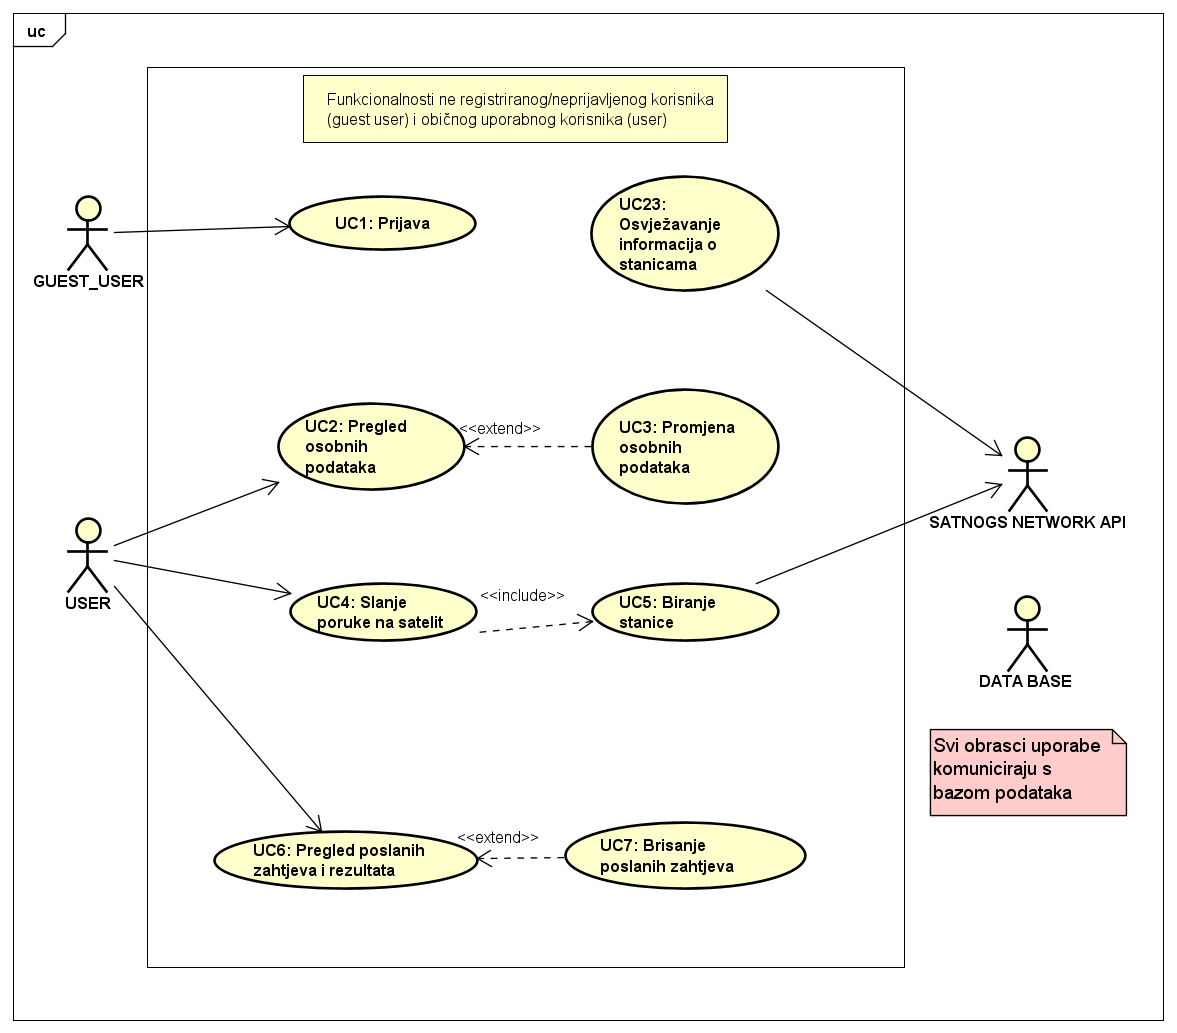
\includegraphics[width=\linewidth]{USECASE1.png}
						\caption{Dijagram obrasca uporabe, funkcionalnost neprijavljenog korisnika i običnog uporabnog korisnika}
						
					\end{figure}
				\begin{figure}[H]
					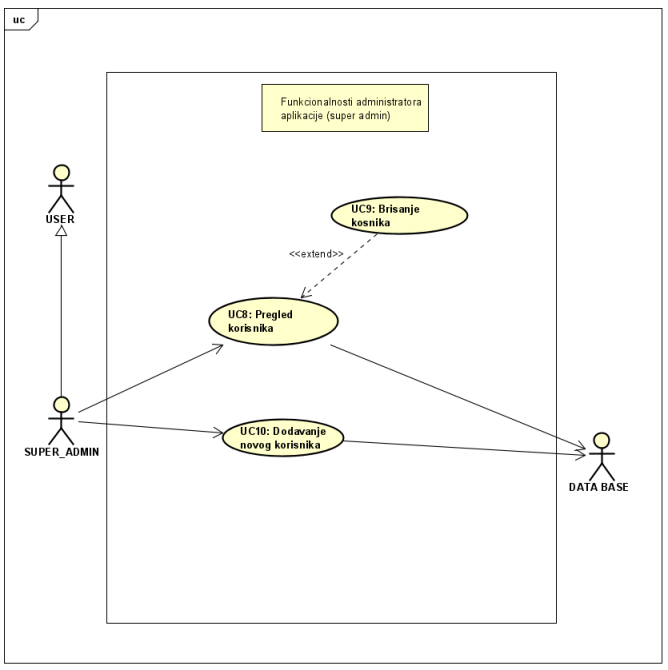
\includegraphics[width=\linewidth]{USECASE2.png}
					\caption{Dijagram obrasca uporabe, funkcionalnost Administratora stranice}
					\label{fig:Dijagrami obrazaca uporabe 8-10}
				\end{figure}
			\begin{figure}[H]
				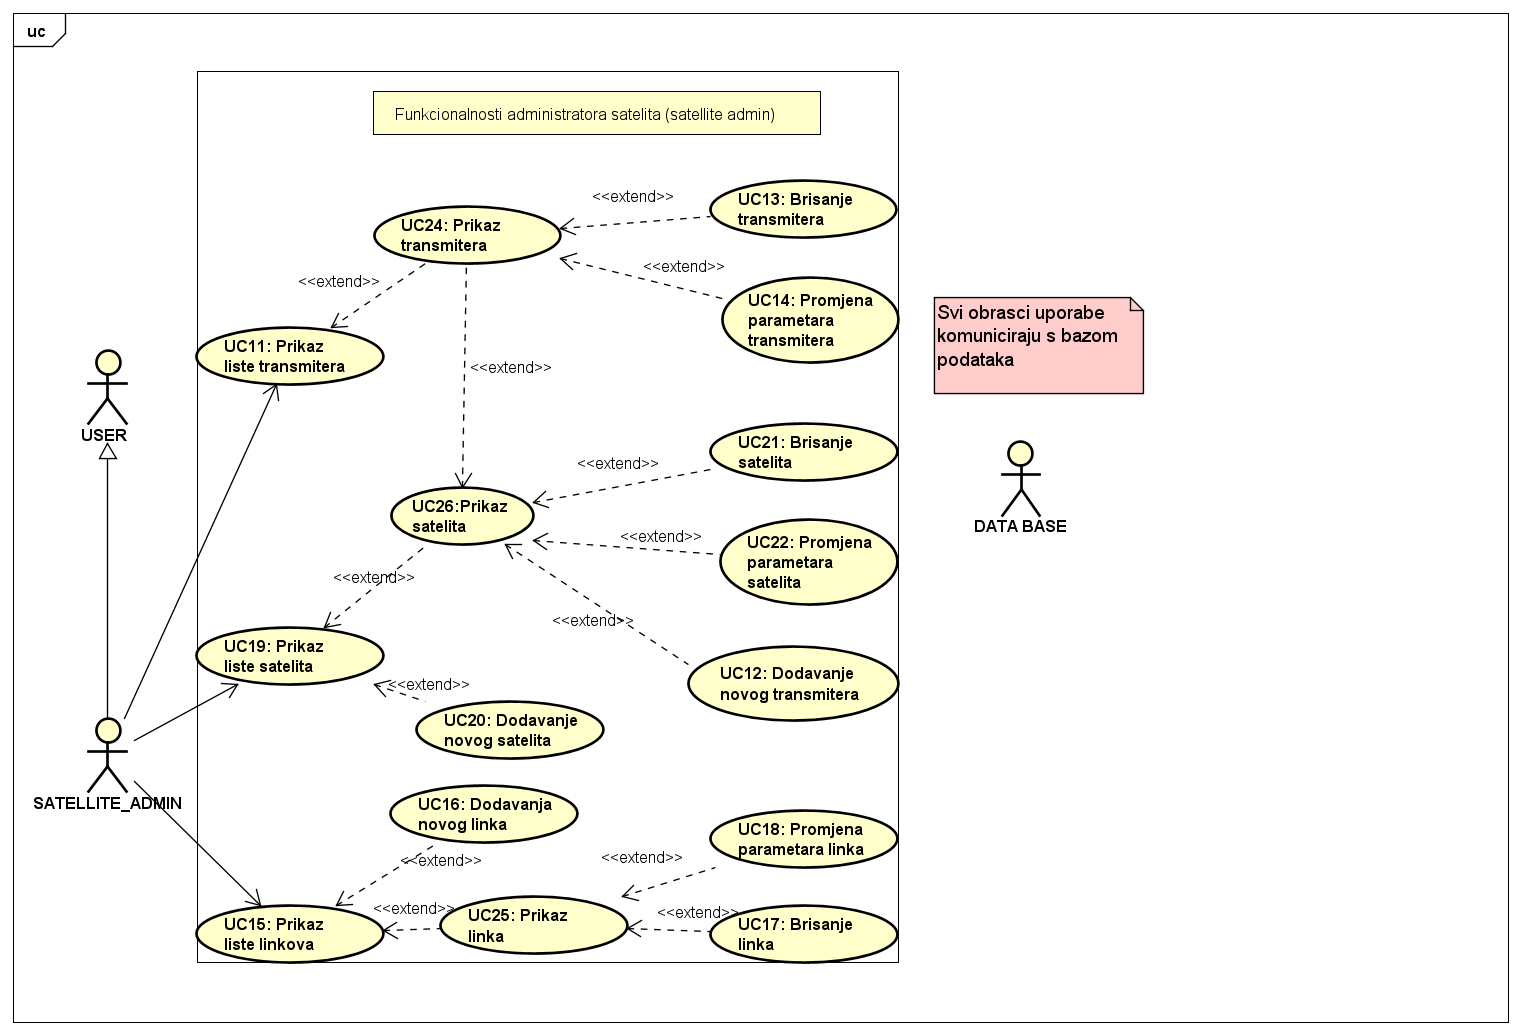
\includegraphics[width=\linewidth]{USECASE3.png}
				\caption{Dijagram obrasca uporabe, funkcionalnost Administratora satelita}
				\label{fig:Dijagrami obrazaca uporabe 11-19}
			\end{figure}
					
				\eject		
				
			\subsection{Sekvencijski dijagrami}
				
\textbf{Obrazac uporabe UC1-Prijava}

{Neregistrirani korisnik upisuje korisničko ime i lozinku. Klikom na gumb "Log in" ti podaci se šalju na validaciju. Ako su uneseni podaci pronađeni u bazi, aplikacija generira token sesije. U suprotnom, šalje se poruka o neispravnoj akreditaciji.}

				\begin{figure}[H]
					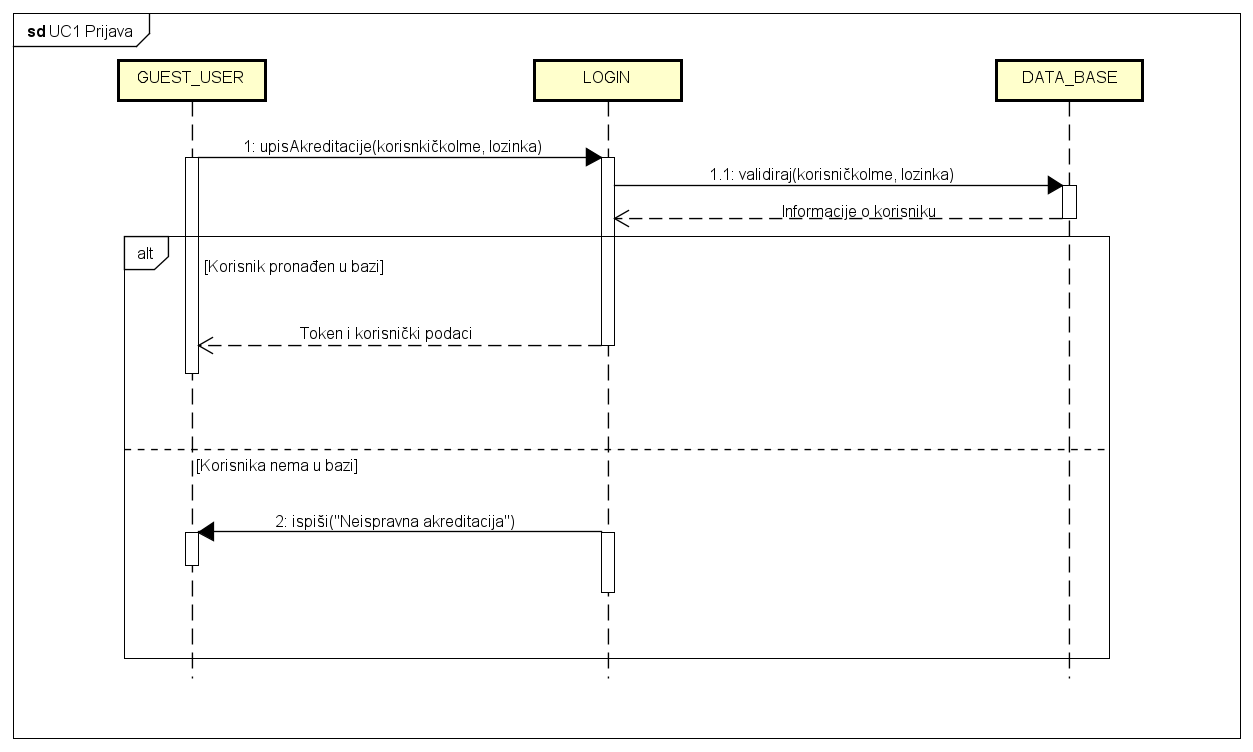
\includegraphics[width=\linewidth]{Sekvencijski1.png}
					\caption{Sekvencijski dijagram prijave korisnika}
					\label{fig:Sekvencijski prijava}
				\end{figure}
			\newpage
			\textbf{Obrazac uporabe UC4-Slanje poruke na satelit}
			
			{Korisnik šalje zahtjev za slanje poruke na satelit. Sustav na taj zahtjev iz baze dohvaća podatke o satelitima te ih šalje natrag korisniku. Korisnik potom bira satelit na koji želi poslati poruku. Aplikacija na taj zahtjev dohvaća listu kompatibilnih linkova za odabrani satelit i šalje ih korisniku. Nakon toga, korisnik odabere jedan link, a zatim se ostvaruje odabir stanice (Vidi \ref{Word:UC5}). Na posljetku, korisnik unosi tekst poruke i pritiskom na gumb "Send" pokreće simulaciju komunikacije sa satelitom. Aplikacija simulira slanje i odgovor koje sprema u bazu, a nakon toga šalje odgovor korisniku. }
		
				\begin{figure}[H]
					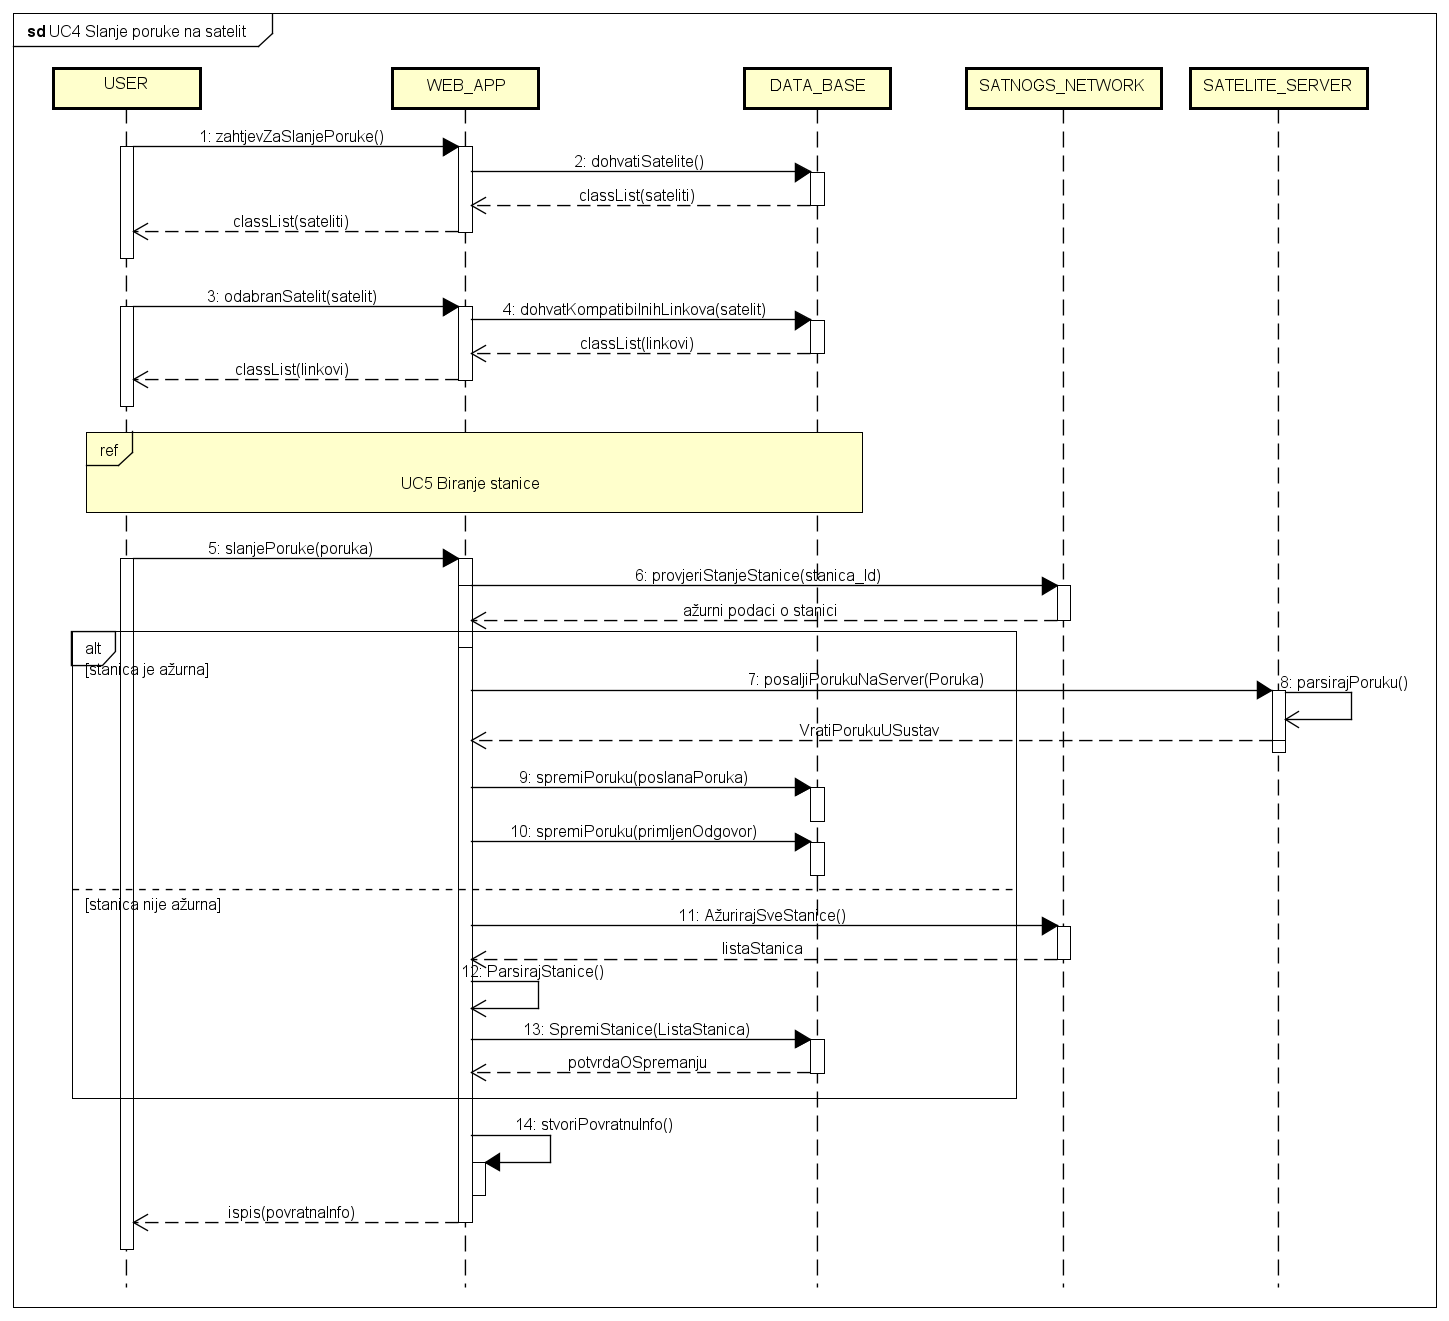
\includegraphics[width=\linewidth]{Sekvencijski2.png}
					\caption{Sekvencijski dijagram slanja poruke}
					\label{fig:Sekvencijski poruka}
				\end{figure}
			\newpage
			\textbf{Obrazac uporabe UC5-Biranje stanice}
			
			{Korisnik odlučuje hoće li odabir stanice prepustiti aplikaciji (automatski) ili samostalno izabrati preko koje stanice će se komunikacija odvijati. Pri odabiru automatske opcije, aplikacija dohvaća iz baze stanice koje su kompatibilne s prethodno odabranim linkom. Odabir optimalne stanice temelji se na atributu broja obzervacija. Iz SatNOGS mreže dohvaćaju se ažurni podaci o odabranoj optimalnoj stanici. Aplikacija uspoređuje podatke o stanici iz baze s dobivenim iz SatNOGS mreže. Ako nije došlo do promjena, korisniku se šalje poruka o pronalasku stanice i on može nastaviti sa slanjem poruke. Ukoliko je došlo do promjena podataka koji utječu na komunikaciju, podaci se u bazi ažuriraju i nastavlja se s traženjem optimalne stanice. U slučaju da stanica više ne postoji u mreži, njen zapis se briše iz baze i ponovno se nastavlja traženje optimalne stanice. \newline
				U drugom slučaju, aplikacija iz baze dohvaća kompatibilne stanice pa šalje upit na SatNOGS mrežu o tim stanicama i po primitku odgovora uspoređuje dobivene podatke s pročitanim podacima iz baze. Ukoliko je došlo do promjena u podacima, ažurira ih u bazi. Zatim, šalje korisniku listu stanice iz koje on treba odabrati željenu stanicu za komunikaciju.}
			
			
				\begin{figure}[H]
					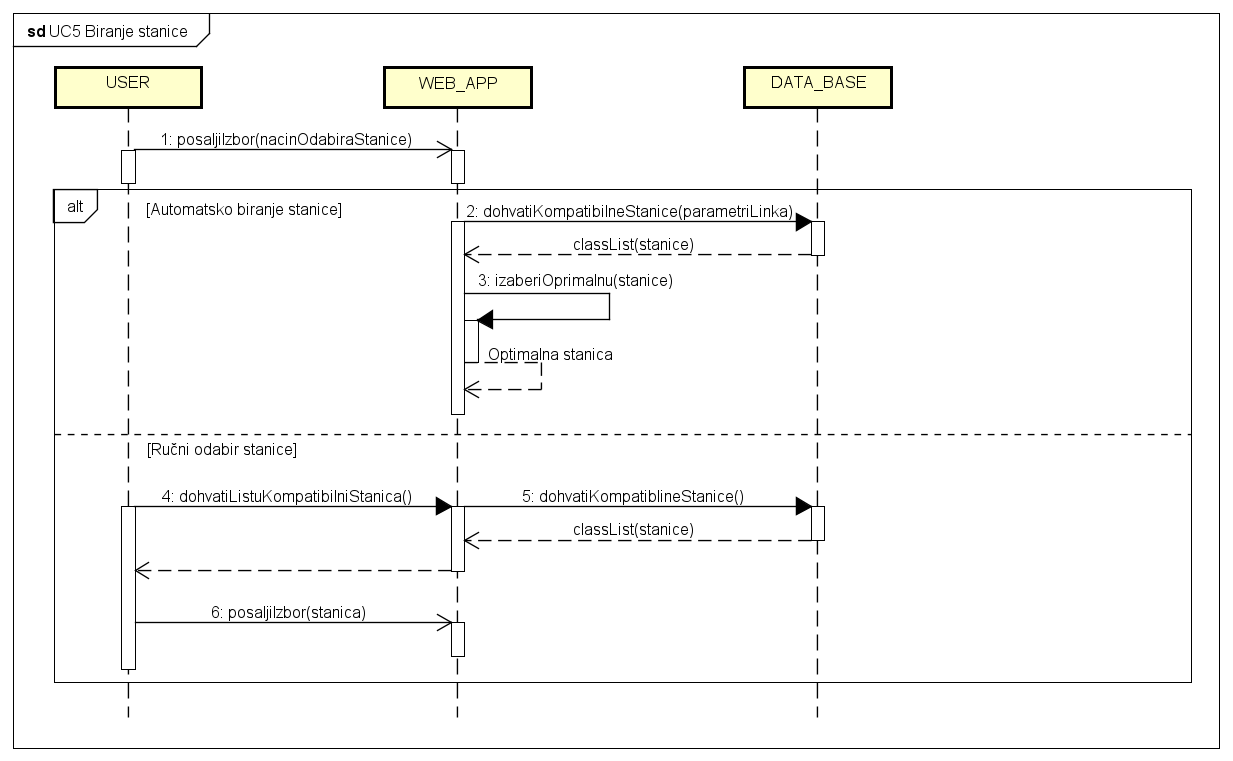
\includegraphics[width=\linewidth]{Sekvencijski3.png}
					\caption{Sekvencijski dijagram biranja stanice}
					\label{fig:Sekvencijski }
				\end{figure}
				
	
		\section{Ostali zahtjevi}
		 
			   \begin{itemize}
                \item Sustav treba biti jednostavan/intuitivan za koristenje, korisnici se moraju znati koristiti sučeljem bez opširnih uputa.
                \item Neispravno korištenje korisničkog sučelja ne smije narušiti funkcionalnost i rad sustava.
                \item Nadogradnja sustava ne smije narušavati postojeće funkcionalnosti sustava.
                \item Lozinke moraju biti kriptirane pri pohrani u bazu.
                \item Sustav treba biti implementiran kao web aplikacija koristeći objektno-\newline orijentirane jezike.
                \item Korisničko sučelje i sustav treba podržavati hrvatske dijakritičke znakove za unos i prikaz tekstualnog sadržaja
                \item Sustavu se treba moći pristupati iz javne mreže pomoću HTTPS
                \item Sustav pri logiranju korisnuku dodjeljuje JWT Token kako bi se garantirao siguran prijenos informacija putem web-a
                \item Sustav omogućava istovremeni rad više korisnika

            \end{itemize}
			 
			 
	